\documentclass[tikz, border=2mm]{standalone}
\usetikzlibrary{calc}
\def\pyramidwidth{0.75cm}
\def\pyramiddepth{0.5cm}
\def\pyramidheight{.35cm}
\def\levels{3}
\def\levelsep{0.05}
\begin{document}
  \sffamily
  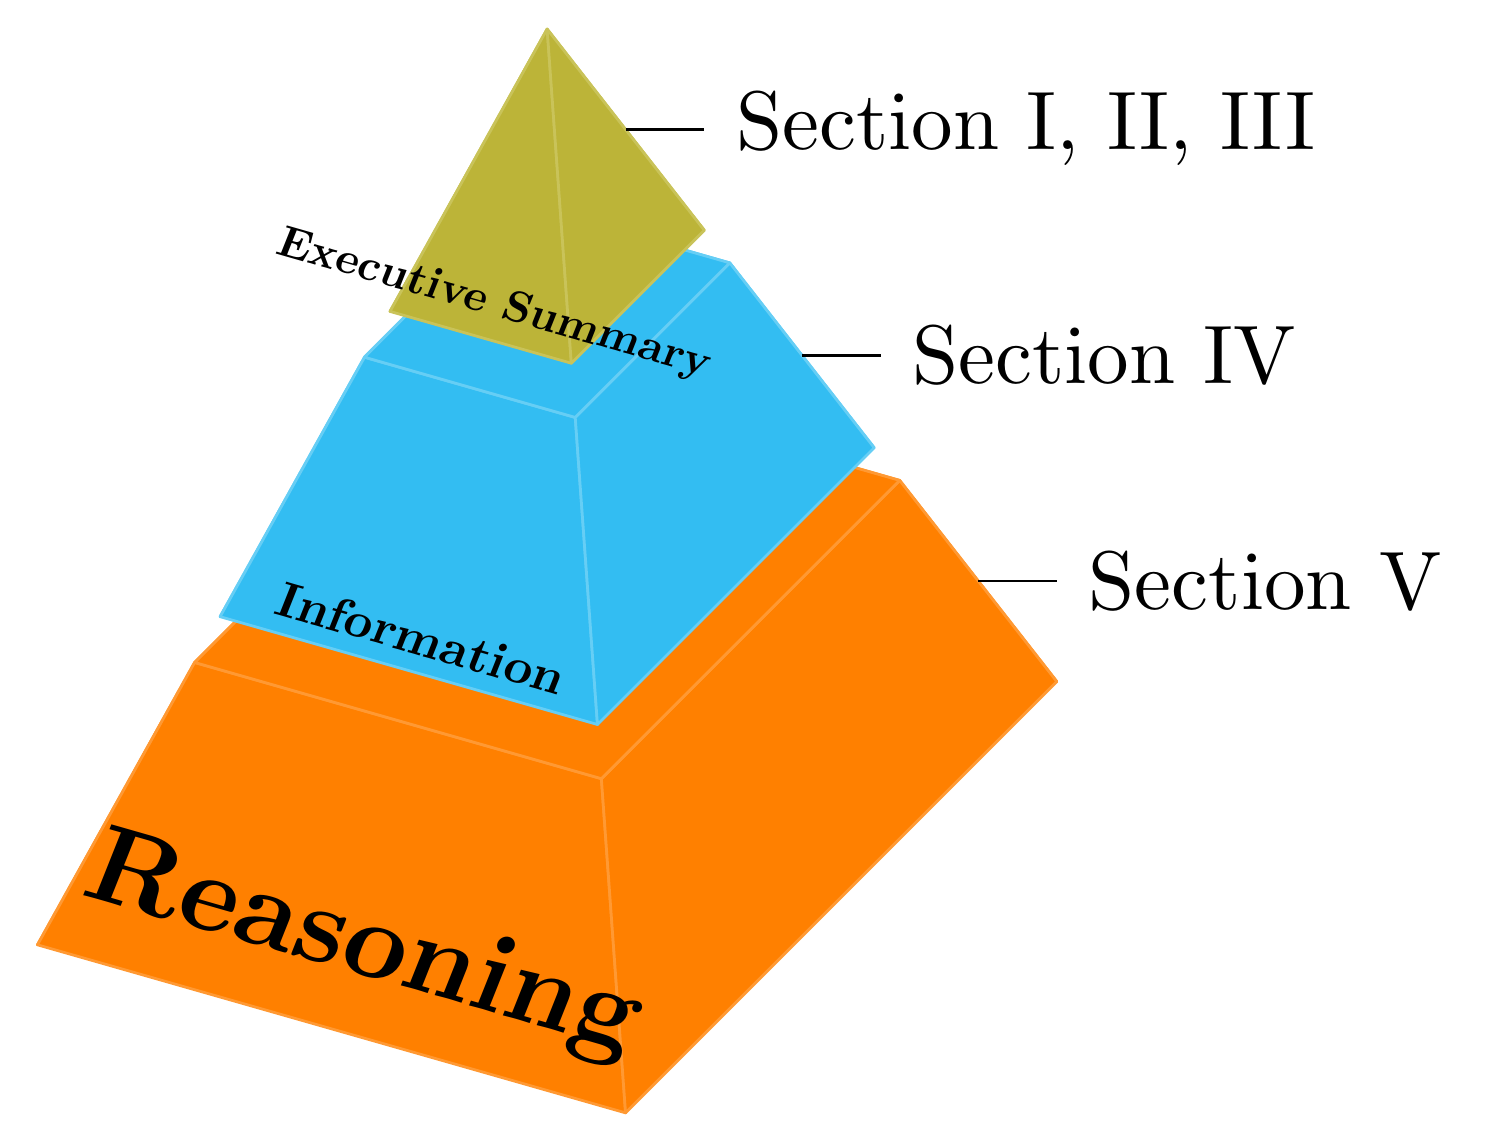
\begin{tikzpicture}[line width=1pt, every node/.style={scale=3},
                      level 1/.style={fill=orange, draw=orange!80},
                      level 2/.style={fill=cyan!80, draw=cyan!60},
                      level 3/.style={fill=yellow!70!black, draw=yellow!70!black!80},
                      x={(3.5mm,-1mm)}]
    \coordinate[alias=A1b] (A) at (0,0,0);
    \coordinate[alias=C1b] (C) at (\pyramidwidth,0,\pyramiddepth);
    \coordinate[alias=B1b] (B) at (0,0,\pyramiddepth);
    \coordinate[alias=D1b] (D) at (\pyramidwidth,0,0);
    \coordinate (H) at (\pyramidwidth/2,\pyramidheight,\pyramiddepth/2);
    \foreach \n in {A,B,C,D}{%
      \foreach \level[remember=\level as \lastlevel (initially 1)] in {2,...,\levels}{%
        \coordinate (\n\lastlevel t) at ($(\n)!\lastlevel/\levels-\levelsep/2!(H)$);
        \coordinate (\n\level b) at ($(\n)!\lastlevel/\levels+\levelsep/2!(H)$);}}
    \foreach \n in {A,B,C,D}{\coordinate (\n\levels t) at (H);}
    \foreach \level in {1,...,\levels}{%
        \foreach \i/\j in {D/A, A/B, B/C, C/D}{%
            \draw[level \level, line join=round] (\i\level b) -- (\j\level b) -- (\j\level t) -- (\i\level t) -- cycle;};
            \draw[level \level, line join=round] (A\level t) -- (B\level t) -- (C\level t) -- (D\level t) -- cycle;};
            
     \begin{scope}[every node/.style={rotate=-16,xslant=.1,above, inner sep=3pt, font=\bfseries}]
       \node[scale=4] at ($(B1b)!.5!(C1b)$) {Reasoning};
       \node[scale=1.8] at ($(B2b)!.5!(C2b)$) {Information};
       \node[scale=1.6] at ($(B3b)!.5!(C3b)$) {Executive Summary};
     \end{scope}
     %
     \begin{scope}[x=1cm]
       \draw ($(D1b)!.5!(D1t)$) -- +(1,0) node[right] {Section V};
       \draw ($(D2b)!.5!(D2t)$) -- +(1,0) node[right] {Section IV};
       \draw ($(D3b)!.5!(D3t)$) -- +(1,0) node[right] {Section I, II, III};
     \end{scope}
  \end{tikzpicture}
\end{document}